\chapter{Feature Scaling}
\label{chap:feature_scaling}

% ========================================
% SECTION 0: METADATA
% ========================================
% Prerequisites: Basic Statistics (Mean, Std Dev)
% Learning Outcomes:
% - Why Euclidean distance breaks with unscaled data
% - Standardization (Z-score) vs Normalization (MinMax)
% - Data Leakage during scaling
% Interview Relevance: High (Practical Implementation)

% ========================================
% SECTION 1: MOTIVATION
% ========================================
\section{Motivation}
Imagine you are predicting House Prices based on two features:
\begin{itemize}
    \item \textbf{Size}: 500 to 5,000 sq ft
    \item \textbf{Bedrooms}: 1 to 5
\end{itemize}

If you calculate the Euclidean distance between two houses:
$$ d = \sqrt{(5000-500)^2 + (5-1)^2} = \sqrt{4500^2 + 4^2} \approx 4500 $$
The distance is almost entirely dominated by the "Size" feature. The number of bedrooms effectively doesn't matter. The algorithm (KNN, SVM, GD) will be biased towards features with larger magnitudes.

% ========================================
% SECTION 2: INTUITION
% ========================================
\section{Intuition: The Elongated Bowl}
For Gradient Descent, unscaled features create an \textbf{elongated cost function surface} (like a long valley).
\begin{itemize}
    \item The gradient is very steep for the large feature and very flat for the small feature.
    \item The optimizer zigs and zags, taking forever to converge.
    \item **Scaled Data** creates a nice circular bowl. The optimizer goes straight to the bottom.
\end{itemize}

% ========================================
% SECTION 3: VISUALIZATION
% ========================================
\section{Visualizing Scaling}

\begin{figure}[h]
    \centering
    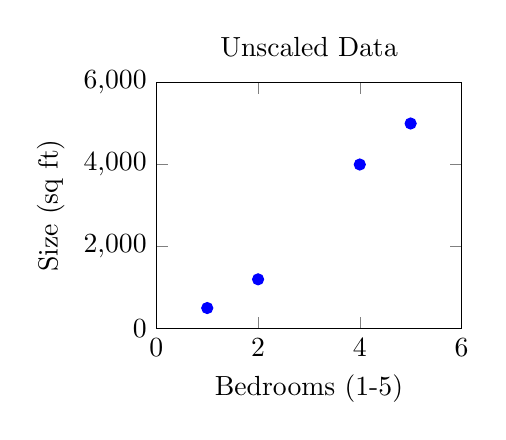
\begin{tikzpicture}
        \begin{axis}[
            title={Unscaled Data},
            xlabel={Bedrooms (1-5)},
            ylabel={Size (sq ft)},
            xmin=0, xmax=6,
            ymin=0, ymax=6000,
            width=0.45\textwidth
        ]
        \addplot[only marks, blue] coordinates {(1, 500) (5, 5000) (2, 1200) (4, 4000)};
        \end{axis}
    \end{tikzpicture}
    \hfill
    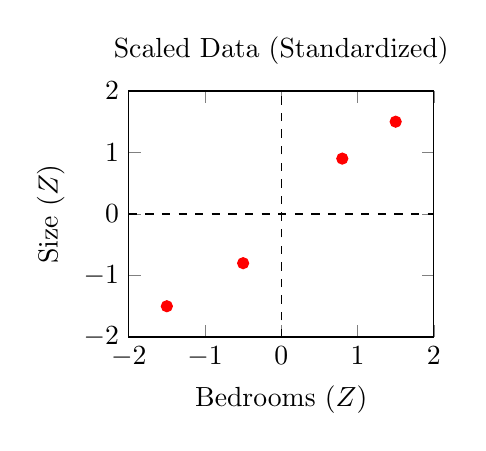
\begin{tikzpicture}
        \begin{axis}[
            title={Scaled Data (Standardized)},
            xlabel={Bedrooms ($Z$)},
            ylabel={Size ($Z$)},
            xmin=-2, xmax=2,
            ymin=-2, ymax=2,
            width=0.45\textwidth
        ]
        \addplot[only marks, red] coordinates {(-1.5, -1.5) (1.5, 1.5) (-0.5, -0.8) (0.8, 0.9)};
        \draw[dashed] (axis cs:0, -2) -- (axis cs:0, 2);
        \draw[dashed] (axis cs:-2, 0) -- (axis cs:2, 0);
        \end{axis}
    \end{tikzpicture}
    \caption{Left: Axis ranges are vastly different. Right: Both axes centered at 0 with similar scale.}
\end{figure}


% ========================================
% SECTION 4: MATHEMATICAL FORMULATION
% ========================================
\section{Methods of Scaling}

\subsection{1. Standardization (Z-Score Normalization)}
Centers data around 0 with unit variance.
$$ Z = \frac{x - \mu}{\sigma} $$
\begin{itemize}
    \item \textbf{Range}: Unbounded (can be $\pm 5$ etc.)
    \item \textbf{Pros}: Handles outliers better than MinMax. Preserves distribution shape.
    \item \textbf{Use Case}: SVM, Logic Regression, Neural Networks (assume Gaussian).
\end{itemize}

\subsection{2. Normalization (Min-Max Scaling)}
Squeezes data into a fixed box $[0, 1]$.
$$ X_{norm} = \frac{x - x_{min}}{x_{max} - x_{min}} $$
\begin{itemize}
    \item \textbf{Range}: STRICTLY $[0, 1]$.
    \item \textbf{Cons}: Very sensitive to outliers. (One billionaire makes everyone else look poor).
    \item \textbf{Use Case}: Image Processing (pixels 0-255), Algorithms requiring fixed range.
\end{itemize}

% ========================================
% SECTION 6: IMPLEMENTATION
% ========================================
\section{Python Implementation}
\begin{lstlisting}[language=Python, caption=StandardScaler vs MinMaxScaler]
from sklearn.preprocessing import StandardScaler, MinMaxScaler
import numpy as np

data = np.array([[500, 1], [5000, 5], [2000, 3]])

# Standardization
scaler = StandardScaler()
print(scaler.fit_transform(data))
# Output: Mean=0, Std=1

# Normalization
minmax = MinMaxScaler()
print(minmax.fit_transform(data))
# Output: Between 0 and 1
\end{lstlisting}

% ========================================
% SECTION 7: PITFALLS (CRITICAL)
% ========================================
\section{Pitfalls: Data Leakage}
\textbf{The Golden Rule}: NEVER fit your scaler on the Test Set.
\begin{itemize}
    \item \textbf{Wrong}: `scaler.fit_transform(X_all)` followed by split.
    \item \textbf{Right}: 
    \begin{enumerate}
        \item Split into Train/Test.
        \item `scaler.fit(X_train)` (Learn mean/std from Train ONLY).
        \item `scaler.transform(X_train)`
        \item `scaler.transform(X_test)` (Use Train's stats to scale Test).
    \end{enumerate}
\end{itemize}

% ========================================
% SECTION 8: INTERVIEW QUESTIONS
% ========================================
\section{HOTS Questions}
\textbf{Q1: Does Decision Tree require feature scaling?}
\begin{itemize}
    \item \textbf{No.} Trees split based on thresholds (e.g., "Is Size > 2000?"). Changing the scale of "Size" (e.g., to meters vs feet) changes the threshold value but not the split point relative to the data.
\end{itemize}

\textbf{Q2: Which scaler should I use if my data has outliers?}
\begin{itemize}
    \item \textbf{RobustScaler} (uses Median and IQR) or StandardScaler. Do NOT use MinMaxScaler, as the outlier will squash the rest of the data into a tiny interval.
\end{itemize}

% ========================================
% SECTION 9: QUICK REFERENCE
% ========================================
\section{Quick Reference Card}

\begin{center}
\fbox{\parbox{0.9\textwidth}{
\textbf{FEATURE SCALING - CHEAT SHEET}
\vspace{0.3cm}

\textbf{Why?}: Distance-based algorithms (KNN, SVM, K-Means) and Gradient Descent fail without it.

\textbf{Formulas}:
\begin{itemize}
    \item \textbf{Standardization}: $Z = \frac{x-\mu}{\sigma}$ (Mean 0, Std 1)
    \item \textbf{MinMax}: $\frac{x-min}{max-min}$ (Range 0-1)
\end{itemize}

\textbf{Algorithm Requirements}:
\begin{center}
\begin{tabular}{|l|l|}
\hline
\textbf{Algorithm} & \textbf{Need Scaling?} \\ \hline
Linear/Log Reg & Yes (for GD convergence) \\ \hline
KNN, K-Means & \textbf{YES!!!!} (Distance check) \\ \hline
SVM & \textbf{YES!!!!} (Margin calculation) \\ \hline
PCA & Yes (Variance based) \\ \hline
Decision Trees & No \\ \hline
Random Forest & No \\ \hline
\end{tabular}
\end{center}

\textbf{Interview Gold}:
\begin{itemize}
    \item \textbf{Leakage}: Fit on Train, Transform on Test.
    \item Trees don't care about scaling.
    \item Outliers destroy MinMaxScaler.
\end{itemize}
}}
\end{center}
